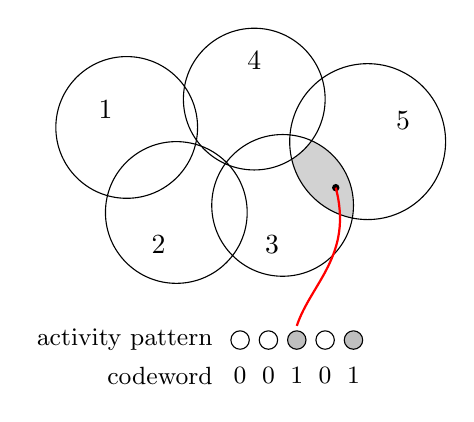
\begin{tikzpicture}[scale=0.9]
  % shaded region: inside fields 3 and 5, outside field 4
  \begin{scope}
    \clip (2.2,0.1) circle (1);
    \clip (3.4,1.0) circle (1.1);
    \fill[gray!35] (0,-1) rectangle (5,3);
    \fill[white] (1.8,1.6) circle (1);
  \end{scope}
  \draw (0,1.2) circle (1);
  \draw (0.7,0) circle (1);
  \draw (1.8,1.6) circle (1);
  \draw (2.2,0.1) circle (1);
  \draw (3.4,1.0) circle (1.1);
  \node at (-0.3,1.45) {$1$};
  \node at (0.45,-0.45) {$2$};
  \node at (1.8,2.15) {$4$};
  \node at (2.05,-0.45) {$3$};
  \node at (3.9,1.3) {$5$};
  \fill (2.95,0.35) circle (1.5pt);
  \draw[red,thick] (2.95,0.35) .. controls (3.2,-0.6) and (2.6,-1.0) .. (2.4,-1.6);
  % activity pattern
  \node[anchor=east,font=\small] at (1.35,-1.8) {activity pattern};
  \foreach \x/\f in {1.6/white,2.0/white,2.4/gray!50,2.8/white,3.2/gray!50}
    \draw[fill=\f] (\x,-1.8) circle (0.13);
  \node[anchor=east,font=\small] at (1.35,-2.3) {codeword};
  \foreach \x/\d in {1.6/0,2.0/0,2.4/1,2.8/0,3.2/1}
    \node[font=\small] at (\x,-2.3) {$\d$};
\end{tikzpicture}
